\documentclass[class=article, crop=false]{standalone}
\usepackage{my_preamble}
\usepackage{pgfplots}
\begin{document}
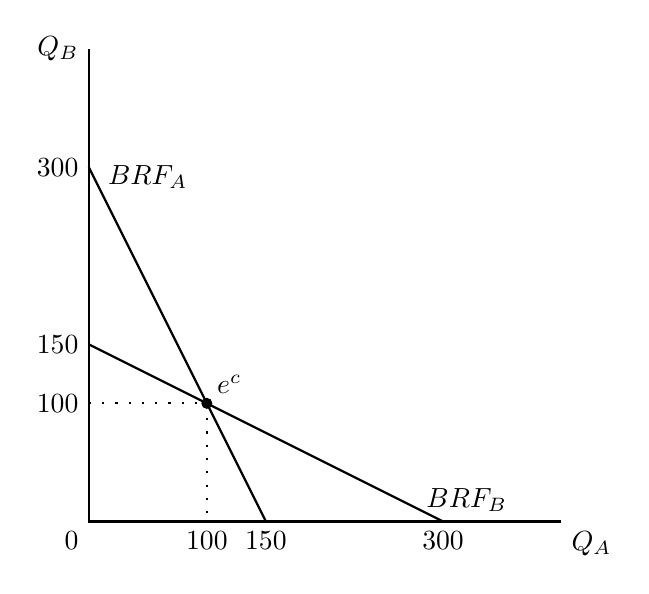
\begin{tikzpicture}[thick,font=\sffamily,scale=1.5]
	%axis
	 \draw (0,4) node[left]{$Q_{B}$} -- (0,0) node[below left] {$0$} 
	  -- (4,0) node[below right]{$Q_{A}$};
	  
	 %BRFs
	\draw[] (0,3) -- (1.5,0); %BRF A
	\draw[] (0,1.5) -- (3,0); %BRF B
	
	%labels
	\node[below] at (0.5,3.1) {$BRF_{A}$}; %BRF A label
	\node[above] at (3.2,0) {$BRF_{B}$}; %BRF B label
	\node[below] at (1.5,0) {$150$}; %A's monopoly quantity
	\node[left] at (0,1.5) {$150$}; %B's monopoly quantity
	\node[below] at (3,0) {$300$}; %PC quantity - A's???
	\node[left] at (0,3) {$300$}; %PC quantity
	
	%equilibria labels
	\node[style={fill=black,circle,inner sep=0pt,minimum size=4pt}] at (1,1) { };
	\node[above right]at (1,1) {$e^{c}$};

	%dotted lines	
	\draw[loosely dotted] (0,1) node[left]{$100$} -| node[pos=0.25,below=3mm] {}
	  (1,0) node[below]{$100$}; %cournot dotted lines
	
\end{tikzpicture}
\end{document}